\chapter{Functional Programming}
\textbf{Functional Programming} languages radicate their roots in the Church's model of computing known as \textbf{\textit{lambda calculus}}.
Such model is based on the notion $\lambda-\textit{parametrized}$ \textit{expressions},
with the focus on defining mathematical functions in a constructive and effective way.
The computation proceeds by substituting parameters into expressions.\nl

Functional programming languages such as \textit{Lisp, Scheme, FP, ML, Miranda} and \textit{Haskell} aim to implement Church's lambda calculus in the form of a programming language which does everything needed by \textbf{composing functions}, thus no \textit{mutable \textbf{state}} and no \textit{side effects}.

{FPL\footnote{Short for \textit{\textbf{F}unctional \textbf{P}rogramming \textbf{L}anguages}} needs some key features which are often absent in \textit{imperative} languages:\ns
\begin{itemize}
   \item $1^{st}$-class order and \textbf{high-order} functions:
   Functions can be \textit{denoted}, passed as \textit{arguments} to other functions, \textit{returned} as result of function invocation
   \item \textbf{Recursion} opposed to \textit{``control variables"}
   \item \textbf{Powerful list facilities}: Recursive functions exploit recursive definition of lists
   \item \textbf{Polymorphism} typically universal parametric
   implicit, 
   which plays a key role when handling containers/collections.
   \item \textbf{Fully general aggregates}:
   there is a wide use of tuples and records,
   besides,
   data structures cannot be modified (\textit{no state!}), they have to be re-created.
   \item \textbf{Structured function returns} allow to pass more meaningful information to the caller, avoiding the need for ``side-effects".
   \item \textbf{Gargabe collection}
\end{itemize}}

% \section*{23 - Ottobre}
\section{FP language families}
\begin{enumerate}
   \item \textbf{LISP}: currently most used for \textit{AI} after Python.
   Original LISP is no longer used, the current standard is \textit{Common LISP} which introduced statical scope opposed to the dynamic one of \textit{Original LISP} ;
   another version is called \textit{Scheme}
   \item \textbf{ML}: Common languages of this family are \textit{Standard ML, Caml,OCaml, F\#}.
   These are compiled languages, but intended for interactive use.
   ML results from the combination of Lisp and Algol-like features, including Garbage collection,
   Abstract data types,
   Module system and
   Exceptions
   \item \textbf{Haskell}: Many features are shared with \textit{ML} languages,
   but with some differences.
   \begin{itemize}
      \item Type inference, Implicit parametric polymorphism, Ad hoc polymorphism (\textbf{overloading}) with type classes
      \item \textbf{Lazy} evaluation, Tail recursion and continuations
      \item \textbf{Purely functional} $\rightarrow$ precise management of side effects
   \end{itemize}
\end{enumerate}
\newpage
\section{Haskell basics}
\begin{paracol}{2}
   \labelitemize{\textbf{\textit{Basic types}}}{
      \begin{itemize}
         \item \texttt{Unit}
         \item \texttt{Booleans}
         \item \texttt{Integers}
         \item \texttt{Strings}
         \item \texttt{Reals}
         \item \texttt{Tuples}
         \item \texttt{Lists}
         \item \texttt{Records}
      \end{itemize}
   }
      \note{
         Note that basic types are written with the first letter Uppercased.
      }
\vspace{\fill}
\switchcolumn
\vspace{\fill}
\labelitemize{\textit{Other types}}{
   \begin{itemize}[label=$\circ$]
      \item Patterns
      \item Declarations
      \item Functions
      \item Polymorphism
      \item Type declarations
      \item Type Classes
      \item Monads
      \item Exceptions
   \end{itemize}
}
\vspace{\fill}
\end{paracol}

Haskell provides an interactive  read-eval-print interpreter (\texttt{ghci}):
many examples are available in the lecture's slides,
here we will discuss only some more interesting ones.

Variables (\textbf{names}) are bound to expressions,
\textit{without }evaluating them (because of \textit{lazy
evaluation}); 
the scope of the binding is the rest of the session.
\lstset{language=Haskell}

\begin{lstlisting}
ghci> let a = 3   -- 'let' can be omitted
ghci> b = a + 2
ghci> b
5
ghci> a = a + 1   -- okay, until here
ghci> a           -- infinite recursion
-- CTRL+C Manual Interrupt
ghci> x = 1:x 
ghci> x           -- infinite ',1' print
\end{lstlisting}


Moving onto \textbf{anonymous functions} i.e. \lstinline|\x -> ...| lambda notation
\begin{lstlisting}
ghci> (\x -> x+1)5      -- apply 5 to anon function
6
ghci> f = (\x -> x+1)
ghci> f 5               -- brackets () can be omitted
6
ghci> h = \(x,y) -> x+y -- tuple Pattern instead of single variable
ghci> h (3,4)           -- brackets are needed here
7
ghci> h 3 4             -- brackets are needed here
-- ERROR
ghci> :t f
f :: Num a => a -> a
ghci> :t h
h :: Num a => (a, a) -> a
\end{lstlisting}

To declare explicit functions instead, the syntax is quite simple
\begin{lstlisting}
f (x,y) = x+y --argument must match pattern (x,y)
\end{lstlisting}

\begin{lstlisting}
   reverse xs =      -- linear, tail recursive
      let rev ( [], accum ) = accum
         rev ( y:ys, accum ) = rev ( ys, y:accum )
      in rev ( xs, [] )
\end{lstlisting}


% \section*{24 - Ottobre}
\section{More on Haskell features}
Let's recall that Haskell is a \textbf{lazy} language,
thus functions and data constructor don't evaluate arguments until they actually need them.

\subsection{List comprehension}

\begin{lstlisting}
   myData = [1,2,3,4,5,6,7]
   twiceData = [2 * x | x <- myData]
   -- [2,4,6,8,10,12,14]
   twiceEvenData = [2 * x| x <- myData, x `mod` 2 == 0]
   -- [4,8,12]
\end{lstlisting}

\begin{lstlisting}
ghci> [ x | x <- [10..20], x /= 13, x /= 15, x /= 19]
      [10,11,12,14,16,17,18,20] -- more predicates
ghci> [ x*y | x <- [2,5,10], y <- [8,10,11]]
      [16,20,22,40,50,55,80,100,110] -- more lists
length xs = sum [1 | _ <- xs] -- anonymous (dont care) var
      -- strings are lists...
removeNonUppercase st = [ c | c <- st, c `elem` ['A'..'Z']]
\end{lstlisting}

\subsection{Datatype declarations}
\begin{lstlisting}
   data Color = Red | Yellow | Blue
   data Atom = Atom String | Number
   data List = Nil | Cons (Atom, List)

   -- General form:
   data <name> = <clause> | ... | <clause>
   <clause> ::= <constructor> | <contructor> <type>
\end{lstlisting}

\begin{lstlisting}
   -- also possible to define Recursive data types
   data Tree = Leaf Int | Node (Int, Tree, Tree)

   Node(4, Node(3, Leaf 1, Leaf 2), Node(5, Leaf 6, Leaf 7))

   -- it is possible to use constructors in pattern matching
   sum (Leaf n) = n
   sum (Node(n,t1,t2)) = n + sum(t1) + sum(t2)
\end{lstlisting}

Besides it is possible to match different cases with a specific \texttt{case} statement;
note that \textbf{Indendation} in case statement \textit{MATTERS}
\begin{lstlisting}
   data Exp = Var Int | Const Int | Plus (Exp, Exp)

   case e of
      Var n -> ...
      Const n -> ...
      Plus(e1,e2) -> ...

   -- Indendation in case statement MATTERS
\end{lstlisting}

\subsection{Function Types}
\lstinline{f :: A -> B} means that:
 \begin{align*}
   \forall x \in A \quad & f(x) =
   \begin{cases}
      \exists y = f(x) \in B \\
      \textit{run forever}
   \end{cases}
\end{align*}
In other words, if $f(x)$ terminates, then $f(x) \in B$.
In ML, functions with type A → B can throw an exception or
have other effects, but \textbf{not} in Haskell.

\subsection{Loops and Recursion}
In FP \texttt{for} and \texttt{while} iterative loops are replaced by \textbf{recusive} subroutines calling themselves directly or indirectly (\textit{mutual recursion}).

\begin{lstlisting}
length' [] = 0
length' (x:s) = 1 + length'(s)
   -- definition using guards and pattern matching
   -- take' n lst returns first n elements of a list
take' :: (Num i, Ord i) => i -> [a] -> [a]
take' n _
| n <= 0 = []
take' _ [] = []
take' n (x:xs) = x : take' (n-1) xs
\end{lstlisting}

\subsection{Higher-Order functions}
Functions that take other functions as arguments or return a function as a result are \textbf{higher-order} functions.

Note also that any curried function with more than one argument is higher-order: applied to one argument it returns a function.

\begin{lstlisting}
applyTwice :: (a -> a) -> a -> a    -- function as arg and res
applyTwice f x = f (f x)

> applyTwice (+3) 10 => 16
> applyTwice (++ " HAHA") "HEY" => "HEY HAHA HAHA"
> applyTwice (3:) [1] => [3,3,1]

applyTwice' f = f.f                 -- equivalent definition
:t (.)
> (.) :: (b -> c) -> (a -> b) -> a -> c
\end{lstlisting}

\begin{lstlisting}
   -- define the operator |> which inverts the order between function and argument
   (|>) a f = f a
   (|>) :: t1 -> (t1 -> t2) -> t2
   -- Seems dull right?
   -- Look at the following example
   
   -- Here, the order of invocation is the same,
   -- but the second "infix" form is (might be) more readable
   > length ( tail ( reverse [1,2,3])) 
      2
   > [1,2,3] |> reverse |> tail |> length 
      2
\end{lstlisting}

\begin{lstlisting}
-- Even these are higher order functions, since they return a function when applied to one argument
(+) :: Num a => a -> a -> a
> let f = (+) 5 // partial application
>:t f ==> f :: Num a => a -> a
> f 4 ==> 9
elem :: (Eq a, Foldable t) => a -> t a -> Bool
> let isUpper = (`elem` ['A'..'Z'])
>:t isUpper ==> isUpper :: Char -> Bool
> isUpper 'A' ==> True
> isUpper '0' ==> False
\end{lstlisting}

\subsection{Combinators}
\lstinline|map| \textit{combinator} applies argument function to each element in
a collection.
\begin{lstlisting}
   map :: (a -> b) -> [a] -> [b]
   map _ [] = []
   map f (x:xs) = f x : map f xs
\end{lstlisting}

\lstinline|filter| takes a collection and a boolean predicate, and
returns the collection of the elements satisfying the
predicate.\\
It is defined as follows:
\begin{lstlisting}
   filter :: (a -> Bool) -> [a] -> [a]
   filter _ [] = []
   filter p (x:xs)
      | p x = x : filter p xs
      | otherwise = filter p xs
\end{lstlisting}
And can be applied in the following way
\begin{lstlisting}
   > filter (>3) [1,5,3,2,1,6,4,3,2,1]
   [5,6,4]
   > filter (==3) [1,2,3,4,5]
   [3]
   > filter even [1..10]
   [2,4,6,8,10]
   > let notNull x = not (null x)
   in filter notNull [[1,2,3],[],[3,4,5],[2,2],[],[],[]]
   [[1,2,3],[3,4,5],[2,2]]
\end{lstlisting}

reduce (\lstinline|foldl|,\lstinline|foldr|): takes a collection, an initial value,
and a binary (two inputs) function , and combines the elements in the
collection according to the function.
Note also that the output  type \lstinline|b| does not necessarily match the input type \lstinline|a| of the initial list, so we can mess around quite a bit \smiley.

\begin{lstlisting}
-- folds values from end to beginning of list
foldr :: Foldable t => (a -> b -> b) -> b -> t a -> b
foldr f z [] = z
foldr f z (x:xs) = f x (foldr f z xs)
-- folds values from beginning to end of list
foldl :: Foldable t => (b -> a -> b) -> b -> t a -> b
foldl f z [] = z
foldl f z (x:xs) = foldl f (f z x) xs
-- variants for non-empty lists
foldr1 :: Foldable t => (a -> a -> a) -> t a -> a
foldl1 :: Foldable t => (a -> a -> a) -> t a -> a
\end{lstlisting}

\begin{paracol}{2}
   
   Let's provide some examples:
   \begin{lstlisting}
      sum = foldr (+) 0
      and = foldr (&&) True
      or = foldr (||) False
      length = foldr (\x -> (+) 1) 0
      length' = foldr (const $ (+) 1) 0 
      -- Here we use const to ignore the first argument
      
      map = foldr ((:) . f) []
   \end{lstlisting}
   
   \switchcolumn

   \begin{figure}[htbp]
      \centering
      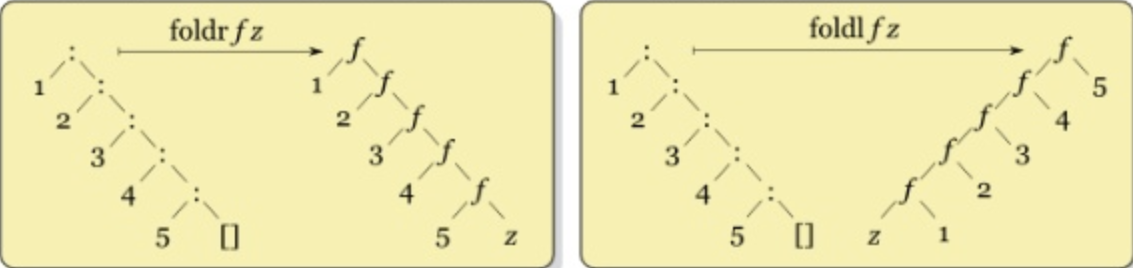
\includegraphics[width=0.95\columnwidth]{images/fold.png}
      \caption{
         The difference between \lstinline|foldl| and \lstinline|foldr| is that the accumulator and element are swapped in the function passed, and that the order of the elements is reversed.
      }
      \label{fig:fold}
   \end{figure}

\end{paracol}
With \lstinline|foldr| we start from the end of the list (we actually recursively go there), and we build up the result from the rightmost element to the leftmost one.
With \lstinline|foldl| instead we start from the beginning of the list and we build up the result from the leftmost element to the rightmost one.

\begin{lstlisting}
   sum' :: (Num a) => [a] -> a
   sum' xs = foldl (\acc x -> acc + x) 0 xs
   
   maximum' :: (Ord a) => [a] -> a
   maximum' = foldr1 (\x acc -> if x > acc then x else acc)
   
   reverse' :: [a] -> [a]
   reverse' = foldl (\acc x -> x : acc) []
   
   product' :: (Num a) => [a] -> a
   product' = foldr1 (*)
   product' = foldr (*) 1
   -- Notice that product' [] returns 1 !

   filter' :: (a -> Bool) -> [a] -> [a]
   filter' p = foldr (\x acc -> if p x then x : acc else acc)[]
   
   head' :: [a] -> a
   head' = foldr1 (\x _ -> x)
   last' :: [a] -> a
   last' = foldl1 (\_ x -> x)
\end{lstlisting}

\subsection{Recursion and Optimization}

From a theoretical point of view recursion and iteration are equivalently expressive,
and typically one is preferred over the other depending on the problem being faced to make the code more intuitive.
In general a procedure call is \textit{much more expensive} than a conditional branch,
however FP compilers can perform many optimizations and produce better code, especially for known blocks;
for this reason the use of combinators such as \lstinline|map,reduce,filter, foreach,...| is strongly encouraged.

\textbf{Tail-recursive} functions are functions in which no operations follow the recursive call(s) in the function,
thus the function returns immediately
after the recursive call,
allowing the compiler to reuse the subroutine's frame on the run-time
stack, since the current subroutine state is no longer needed.
Besides many compilers instead of re-invoking the function,
simply jump to the beginning of the function.

Let's provide the classic example of Fibonacci to illustrate how to convert a normal recursive function to its tail-recursive correspondant one:
\begin{lstlisting}
   -- typical Fibonacci
   fib = \n -> if n == 0 then 1
      else if n == 1 then 1
         else fib (n - 1) + fib (n - 2)
   
   fibTR = \n -> let fibhelper (f1, f2, i) =
      if (n == i) then f2
         else fibhelper (f2, f1 + f2, i + 1)
      in fibhelper(0,1,0)
\end{lstlisting}
Notice that \lstinline|fibTR| takes only $\mathcal{O}(n)$ since it builds the Fibonacci sequence starting from 1 to $n$,
while the more canonical approach calculates multiple times the same values,
and starts from $n$ until 1 is reached.

\lstinline|foldl| is tail-recursive, \lstinline|foldr| is not. But because of
laziness Haskell has \textbf{no} tail-recursion optimization.
Despite this, it provides a more efficient variant of foldl called \lstinline|foldl'| where f is evaluated \textbf{strictly}.\\
\textit{Strictly} means that the compiler evaluates the accumulator at \textit{each step} of the folding process, ensuring that intermediate values are not built up as \textit{unevaluated thunks} i.e. Haskell's term for delayed computations.
Due to its \textit{strictness} \lstinline|fold'| is less likely to cause \textbf{space leaks} (see note below), and it generally has better performance for many common folding operations.

\note{\textbf{``Space leaks''} may happen when a program retains references to data that should no longer be needed, preventing the garbage collector from reclaiming memory. 
This can lead to inefficient memory usage and, in some cases, cause the program to run out of memory.
This (generally) occurs only when handling large data sources or \textit{infinite data structures} (which are allowed in Haskell);
space leaks may be very hard to debug,
tools like memory profilers and heap profiling can be helpful in identifying them}